\section{Análise da Correlação entre as Taxas de \textit{Upload} e \textit{Download} para os Horários com o Maior Valor de Tráfego}

Nesta seção, foi analisada a relação entre as taxas de \textit{upload} e \textit{download} para os horários de maior tráfego identificados previamente. Para isso, foram calculados os coeficientes de correlação amostral e gerados gráficos de dispersão (\textit{scatter plots}) comparando as taxas de \textit{upload} e \textit{download} para os dispositivos \textit{Smart-TV} e \textit{Chromecast}.

\subsection{Cálculo do Coeficiente de Correlação}

O coeficiente de correlação de Pearson foi calculado para cada dispositivo, utilizando o método \texttt{corr} da biblioteca \texttt{pandas} do Python. O coeficiente de correlação varia de -1 a 1, onde valores próximos de 1 indicam uma correlação positiva forte, valores próximos de -1 indicam uma correlação negativa forte e valores próximos de 0 indicam ausência de correlação.

considerando os datasets correspondentes aos horários selecionados:
\begin{itemize}
    \item \textbf{\textit{Smart-TV}:} Comparação entre o Dataset 1 (\textit{Upload}) e o Dataset 2 (\textit{Download}).
    \item \textbf{\textit{Chromecast}:} Comparação entre o Dataset 3 (\textit{Upload}) e o Dataset 4 (\textit{Download}).
\end{itemize}

Os valores dos coeficientes de correlação para cada dispositivo são apresentados na Tabela~\ref{tab:coeficientes_correlacao}.

\begin{table}[H]
    \centering
    \caption{Coeficientes de correlação amostral entre as taxas de \textit{upload} e \textit{download}.}
    \label{tab:coeficientes_correlacao}
    \begin{tabular}{|c|c|}
        \hline
        \textbf{Dispositivo} & \textbf{Coeficiente de Correlação} \\ \hline
        \textit{Smart-TV} & 0.9156 \\ \hline
        \textit{Chromecast} & 0.2248 \\ \hline
    \end{tabular}
\end{table}

\subsection{Gráficos de Dispersão}

Os gráficos de dispersão foram gerados para ilustrar a relação entre as taxas de \textit{upload} e \textit{download} para os dois dispositivos. Esses gráficos estão apresentados na Figura~\ref{fig:scatter_plot}.

\begin{figure}[H]
    \centering
    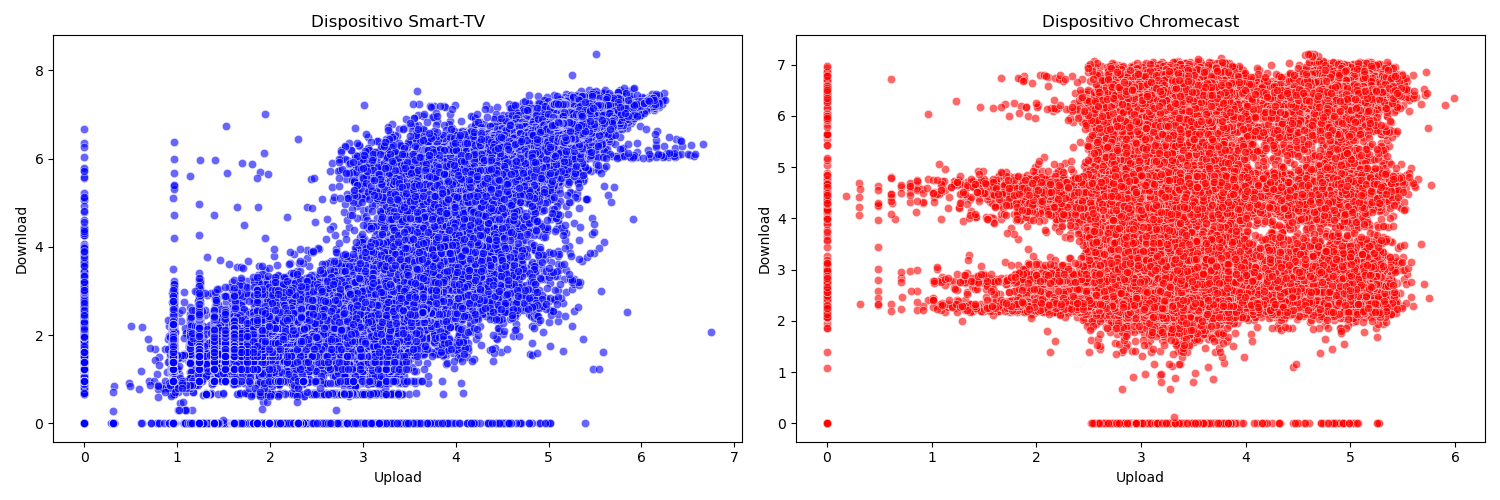
\includegraphics[width=0.8\textwidth]{../correlação/scatter_plot.png}
    \caption{Gráficos de dispersão entre as taxas de \textit{upload} e \textit{download} para os dispositivos \textit{Smart-TV} e \textit{Chromecast}.}
    \label{fig:scatter_plot}
\end{figure}

\subsection{Análise dos Resultados}

Os resultados apresentados demonstram padrões distintos na relação entre as taxas de \textit{upload} e \textit{download} para os dispositivos \textit{Smart-TV} e \textit{Chromecast}. 

Para a \textit{Smart-TV}, o coeficiente de correlação de 0.9156 indica uma forte relação positiva entre as taxas de \textit{upload} e \textit{download}. Esse comportamento é evidenciado no gráfico de dispersão (Figura~\ref{fig:scatter_plot}), onde os pontos formam um padrão alinhado, sugerindo que aumentos em uma taxa estão fortemente associados a aumentos na outra. A concentração dos pontos reflete também a homogeneidade dos dados durante o horário analisado, reforçando a sincronização entre os \textit{datasets} 1 e 2, uma vez que os horários de maior tráfego coincidem (20h para ambos).

Por outro lado, o \textit{Chromecast} apresentou um coeficiente de correlação de 0.2248, indicando uma relação positiva fraca entre as taxas de \textit{upload} e \textit{download}. No gráfico de dispersão, os pontos estão significativamente mais espalhados, sugerindo uma menor dependência entre as duas taxas. Esse comportamento pode ser atribuído à falta de sincronização entre os horários analisados nos \textit{datasets} 3 e 4 (22 e 23h, respectivamente), o que resulta em padrões de tráfego menos alinhados.

\subsection{Análise dos Resultados}

Os resultados apresentados demonstram padrões distintos na relação entre as taxas de \textit{upload} e \textit{download} para os dispositivos \textit{Smart-TV} e \textit{Chromecast}.

Para a \textit{Smart-TV}, o coeficiente de correlação de 0.9156 reflete uma relação positiva forte entre as taxas de \textit{upload} e \textit{download}. Esse comportamento é evidenciado no gráfico de dispersão (Figura~\ref{fig:scatter_plot}), onde os pontos se alinham de forma consistente, sugerindo que aumentos em uma taxa estão fortemente associados a aumentos na outra. Essa relação linear clara é favorecida pela coincidência nos horários analisados (20h para ambos os \textit{datasets}), indicando sincronização nos padrões de tráfego. Essa forte correlação é importante para o provedor, pois permite otimizar recursos simultaneamente para \textit{upload} e \textit{download} em horários de pico.

Por outro lado, o \textit{Chromecast} apresentou um coeficiente de correlação de 0.2248, indicando uma relação positiva fraca entre as taxas. No gráfico de dispersão, os pontos aparecem significativamente mais espalhados, refletindo menor dependência entre \textit{upload} e \textit{download}. Esse comportamento pode ser atribuído ao desalinhamento entre os horários analisados (22h para \textit{upload} e 23h para \textit{download}), o que diminui a sincronização entre os padrões de tráfego. Essa diferença entre os dispositivos sugere que, para o \textit{Chromecast}, a alocação de recursos deve ser feita de forma independente para cada taxa.

É importante notar que a correlação de Pearson utilizada mede apenas relações lineares. Embora a \textit{Smart-TV} apresente uma correlação alta, e o \textit{Chromecast}, uma correlação baixa, outros padrões de dependência não lineares podem estar presentes e não foram capturados nesta análise. Estudos futuros podem considerar métodos como correlações não paramétricas ou análises de causalidade para uma compreensão mais abrangente.

Esses resultados possuem implicações práticas significativas. Para a \textit{Smart-TV}, estratégias de gerenciamento de tráfego podem se beneficiar de uma abordagem integrada para \textit{upload} e \textit{download}, especialmente em horários de pico. Para o \textit{Chromecast}, a menor correlação sugere a necessidade de monitoramento e alocação de recursos separados para cada tipo de tráfego. Além disso, a sincronização dos horários analisados pode ser explorada em estudos futuros para aumentar a precisão e relevância das análises de correlação.
